\chapter{Copy Protection Status Quo}
\label{chapter:copy_protection_status_quo}

Like introduced in \autoref{chapter:android_status_quo} there
are different goals of copy protection mechanisms starting from
preventing reverse code engineering to protect intellectual property
and reaching to hinder patching to get prohibited access.
The common denominator of those goals is the protection of
the DEX file of every app. A variety of tools do exist that
are able to transform DEX into different readable formats,
modify it and repack it again since the DEX contains
a lot of meta data for its contents (classes, methods, \ldots)
\parencite{dex}.


\section{DEX Dissassembly and Repackaging}
Generally there do exist two possible outcomes of DEX disassembling
- Java code (\code{*.java}) and Smali code (\code{*.smali}).
Since the DEX format is more or less just a different mapping of a
JAR and its containing \code{.class} files, the transition to JAR
is quite simple \parencite{dvminternals}. A tool that is able to
perform this step is ``dex2jar'' \parencite{dex2jartool}.
Along with this JAR, standard Java decompiler like ``JD-GUI''
\parencite{jdtool} can be used to produce the \code{*.java} source code.
If the \code{*.java} is supposed to change and repacked, it can
be again compiled into JAR with Oracle's ``javac'' \parencite{javactool}
followed by Googles ``dx'' tool \parencite{dxtool}
to produce the manipulated DEX.

The alternative way is the use of ``smali/baksmali'' tool
\parencite{smalitool} which is a direct assembler and disassembler
for DEX files rather than taking the Java code detour. There is also
a tool included that can convert the ODEX back to DEX.

Overall, the dissassembly of unchanged DEX is quite easy and is shown
as a concluding overview in \autoref{fig:dex_disassembly}

Therefore several countermeasures were established which are
described in the following sections.

\begin{figure}[htb]
  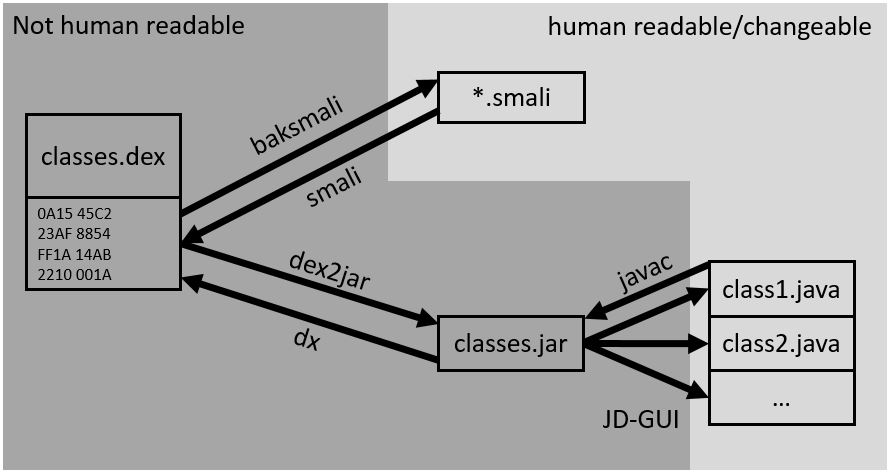
\includegraphics[width=\textwidth]{figures/dex_disassembly}
  \caption[DEX Assembly/Disassembly]{DEX Assembly/Disassembly}
  \label{fig:dex_disassembly}
\end{figure}


\section{Obfuscation Techniques}
Obfuscation in the context of copy protection for application
is generally the term for hardening an application against
reverse code engineering techniques. It can be achieved by different methods
that can be separated in two main groups, static and dynamic obfuscation.
Static means that the obfuscation technique is applied to code units (source
code, binaries, ...) while the application is not executed. Therefore an
attacker could possibly successful analyze the application without executing it
if he manages to break this obfuscation. Applications that are dynamically
obfuscated on the other hand, are much harder to analyze. The behavior
of the application is not decided until its execution. An attacker needs to connect to the process of the running application followed by a just in time inspection.

It does follow a list of common static and dynamic obfuscation techniques
for Android applications. However, this list is mainly focussed on
the Dalvik runtime since ART has been released quite recently.
Where static obfuscation techniques do show the same behavior in both
runtimes, the dynamic solutions do possibly not since the exeuction process
of apps in ART does differ (described in \autoref{section:app_execution}).
The impact of those techniques to ART will get analyzed in a later chapter.
Therefore, the techniques given below are supposed to be an outline to
the topic of copy protection mechanisms.


\subsection{Static}
\subsubsection{Common Source Code Obfuscation}
The most common and simple way of harden source code is to remove any kind of meta data
that has been added during the development process. Means destroying/modifying
information that originally was present in the source code.
Possible prospects to do this are the renaming of string identifiers of
classes, variables, methods and functions, to artificially insert
irreducible code, create artificial parallelization, perform method inlining/outlining, to unroll loops, encoding strings or changing the control flow in
order to confuse code analysts by keeping the original behavior
\parencite{lvl_imp}.

Popular tools for that purpose are Google's ``ProGuard''
\parencite{proguardtool} which is included in the Android build system and
can be enabled easily as well as``DexGuard'' by GuardSquare
\parencite{dexguardtool}. ``ProGuard'' does
operate on source code level where ``DexGuard'' operates on DEX.
Since the first ``layer'' of Android applications is Java code, classical Java
obfuscators also can be used.

\subsubsection{Junk-Byte-Insertion}
Junk-Byte-Insertion's goal is to prohibit the use of static analyzing
disassembling tools. It does work for tools using the
``linear sweep'' method to analyze a file. That means
the tools are processing every instruction from the entry-point
till the end without interpreting them (e.g. not following jumps).
That examining technique can be exploited to break the disassembling
procedure. Let's assume we do have the code snippet of
\autoref{fig:junk_byte_listening}
on source code level.

\begin{figure}[htb]
  \centering
  \begin{tabular}{c}
  \begin{lstlisting}[language=Java]
    if (false) {
        insertBytes();
    } else {
        proceedProgram();
    }
  \end{lstlisting}
  \end{tabular}
  \caption[Junk-Byte-Insertion]{Junk-Byte-Insertion Example}
  \label{fig:junk_byte_listening}
\end{figure}

Cause of the if-condition, the \code{insertBytes()} method is never
reached. Since ``linear sweep'' does not perform jumps, the analyzing tool
is trying to also revert the following instructions into source code. By choosing a specific sequence of bytes, the transformation will fail.

Enhanced tools will use the ``recursive traversal'' technique to analyze a
file which is capable of detecting dead branches and conditional jumps like in the example above.
These tools also may be tricked by choosing a more complicated condition for
if-conditions that can only be evaluated at runtime and therefore the
whole conditional branch (including the breaking byte sequence) would also tried to be evaluated (Actually this technique does already count to dynamic obfuscation).
\parencite{lvl_imp}.

\subsection{Dynamic}
\subsubsection{Hidden Methods Invocation}
In \parencite{lvl_imp} a technique is described to hide a whole method
in \code{.dex} files. This hiding method is highly dependent on the DEX specification from Google \parencite{dex} that will be analyzed in detail
later in this thesis.
It does base on the fact that the actual instructions of methods residing
in the \code{data} section of a DEX are referenced from another section.
These references (which are offsets into the data section) can be faked
to hide specific methods when the DEX gets parsed
(showed in \autoref{fig:hidden_method_invocation}) In order to achieve
this effect, a few bytes obviously need to be changed.
Since the DEX format also does include a checksum to be resistant
against transmission errors, a revaluation is also necessary.
After that hiding step, the method is invisible for static analyzing tools
as well as for the DVM itself. Thats why the changes to the DEX need to
be reversed at runtime. The own DEX file must be loaded into a byte array
followed by reverting the changes and Java reflection to execute it.

\begin{figure}[htb]
  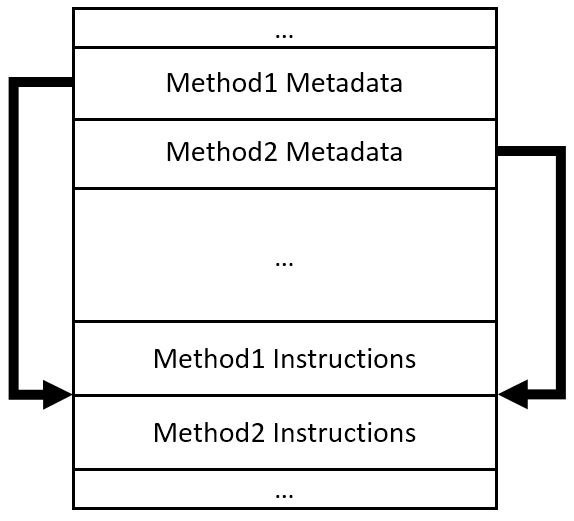
\includegraphics[width=\textwidth]{figures/hidden_method_invocation}
  \caption[Hidden Methods Invocation]{Hidden Methods Invocation Principle}
  \label{fig:hidden_method_invocation}
\end{figure}

\subsubsection{Dynamic Code Loading}
The principle of Dynamic Code Loading is to reveal the actual program code
not before running the application. This behavior can be achieved by
implementing a stub application that will load the actual application file
(in case of Android that would be the DEX) followed by execution.
That file can either can be distributed encrypted within the app stored
in the \code{assets} folder or it can be fetched from a server.
Android does provide a public method within
the \code{DexFile} class to dynamically load DEX files
(\code{openDexFile(String sourceName, String outputName, int flags)})
and loading included classes \parencite{dexfileclass}. The side effect
of the \code{openDexFile()} call is the created ODEX that gets saved and
can't be deleted afterwards because of missing app permissions.
That file persists after closing the application and therefore
it can be analyzed again with static methods. In \parencite{code_protection},
a circumvention to that problem is described by using the JNI.
The \code{libdvm.so} library does offer a private method to open DEX files
that does accept DEX content in form of a byte array.
By establishing this own JNI implementation of
\code{openDexFile(byte[]content)} the loaded dex file is only present
in volatile memory and does not create an ODEX \parencite{code_protection}.

\subsubsection{Self Modifying Code}

